% !TEX root = ../../main.tex

% --------------------------------------
% labels: \label{mil3:res:[type]:[name]}
% --------------------------------------
% PAST TENSE


From this point and onwards (Sects.~\ref{sec:mil3} \&~\ref{sec:mil4}), the results were obtained \emph{after} reproducing the background with $N\ped{eff}=0$. This caused some changes in numerical values for e.g.~radiation-matter equality, but did not change the important results and takeaways from the previous work (Sects.~\ref{sec:mil1} \&~\ref{sec:mil2}). 


The figures below demonstrate our results for three wave numbers $k\in\{k_l, k_i, k_s\}$. We chose $k_l\equiv0.001\unit{Mpc}^{-1}$ to represent the large-scale modes and $k_s\equiv0.1\unit{Mpc}^{-1}$ for the small-scales. The intermediate-scale modes are represented by $k_i\equiv0.01\unit{Mpc}^{-1}$. We noted that $k_i\approx k\ped{eq}= 0.0115\unit{Mpc}^{-1}$. For relevant details, see~\cref{mil3:res:tab:wavenumbers}. We stress that the time of horizon entry is merely a definition, and is at best a naive estimate of when a mode succumbs to causal physics.

We present the absolute values of the matter and energy perturbations in the upper panels of~\cref{mil3:res:fig:matter_perturbations}. The lower panels of said figure emphasise the oscillations around zero of the density and velocity perturbations for the photons.
\begin{figure*}[!ht]
    \begin{subfigure}{0.49\linewidth}
        \centering
        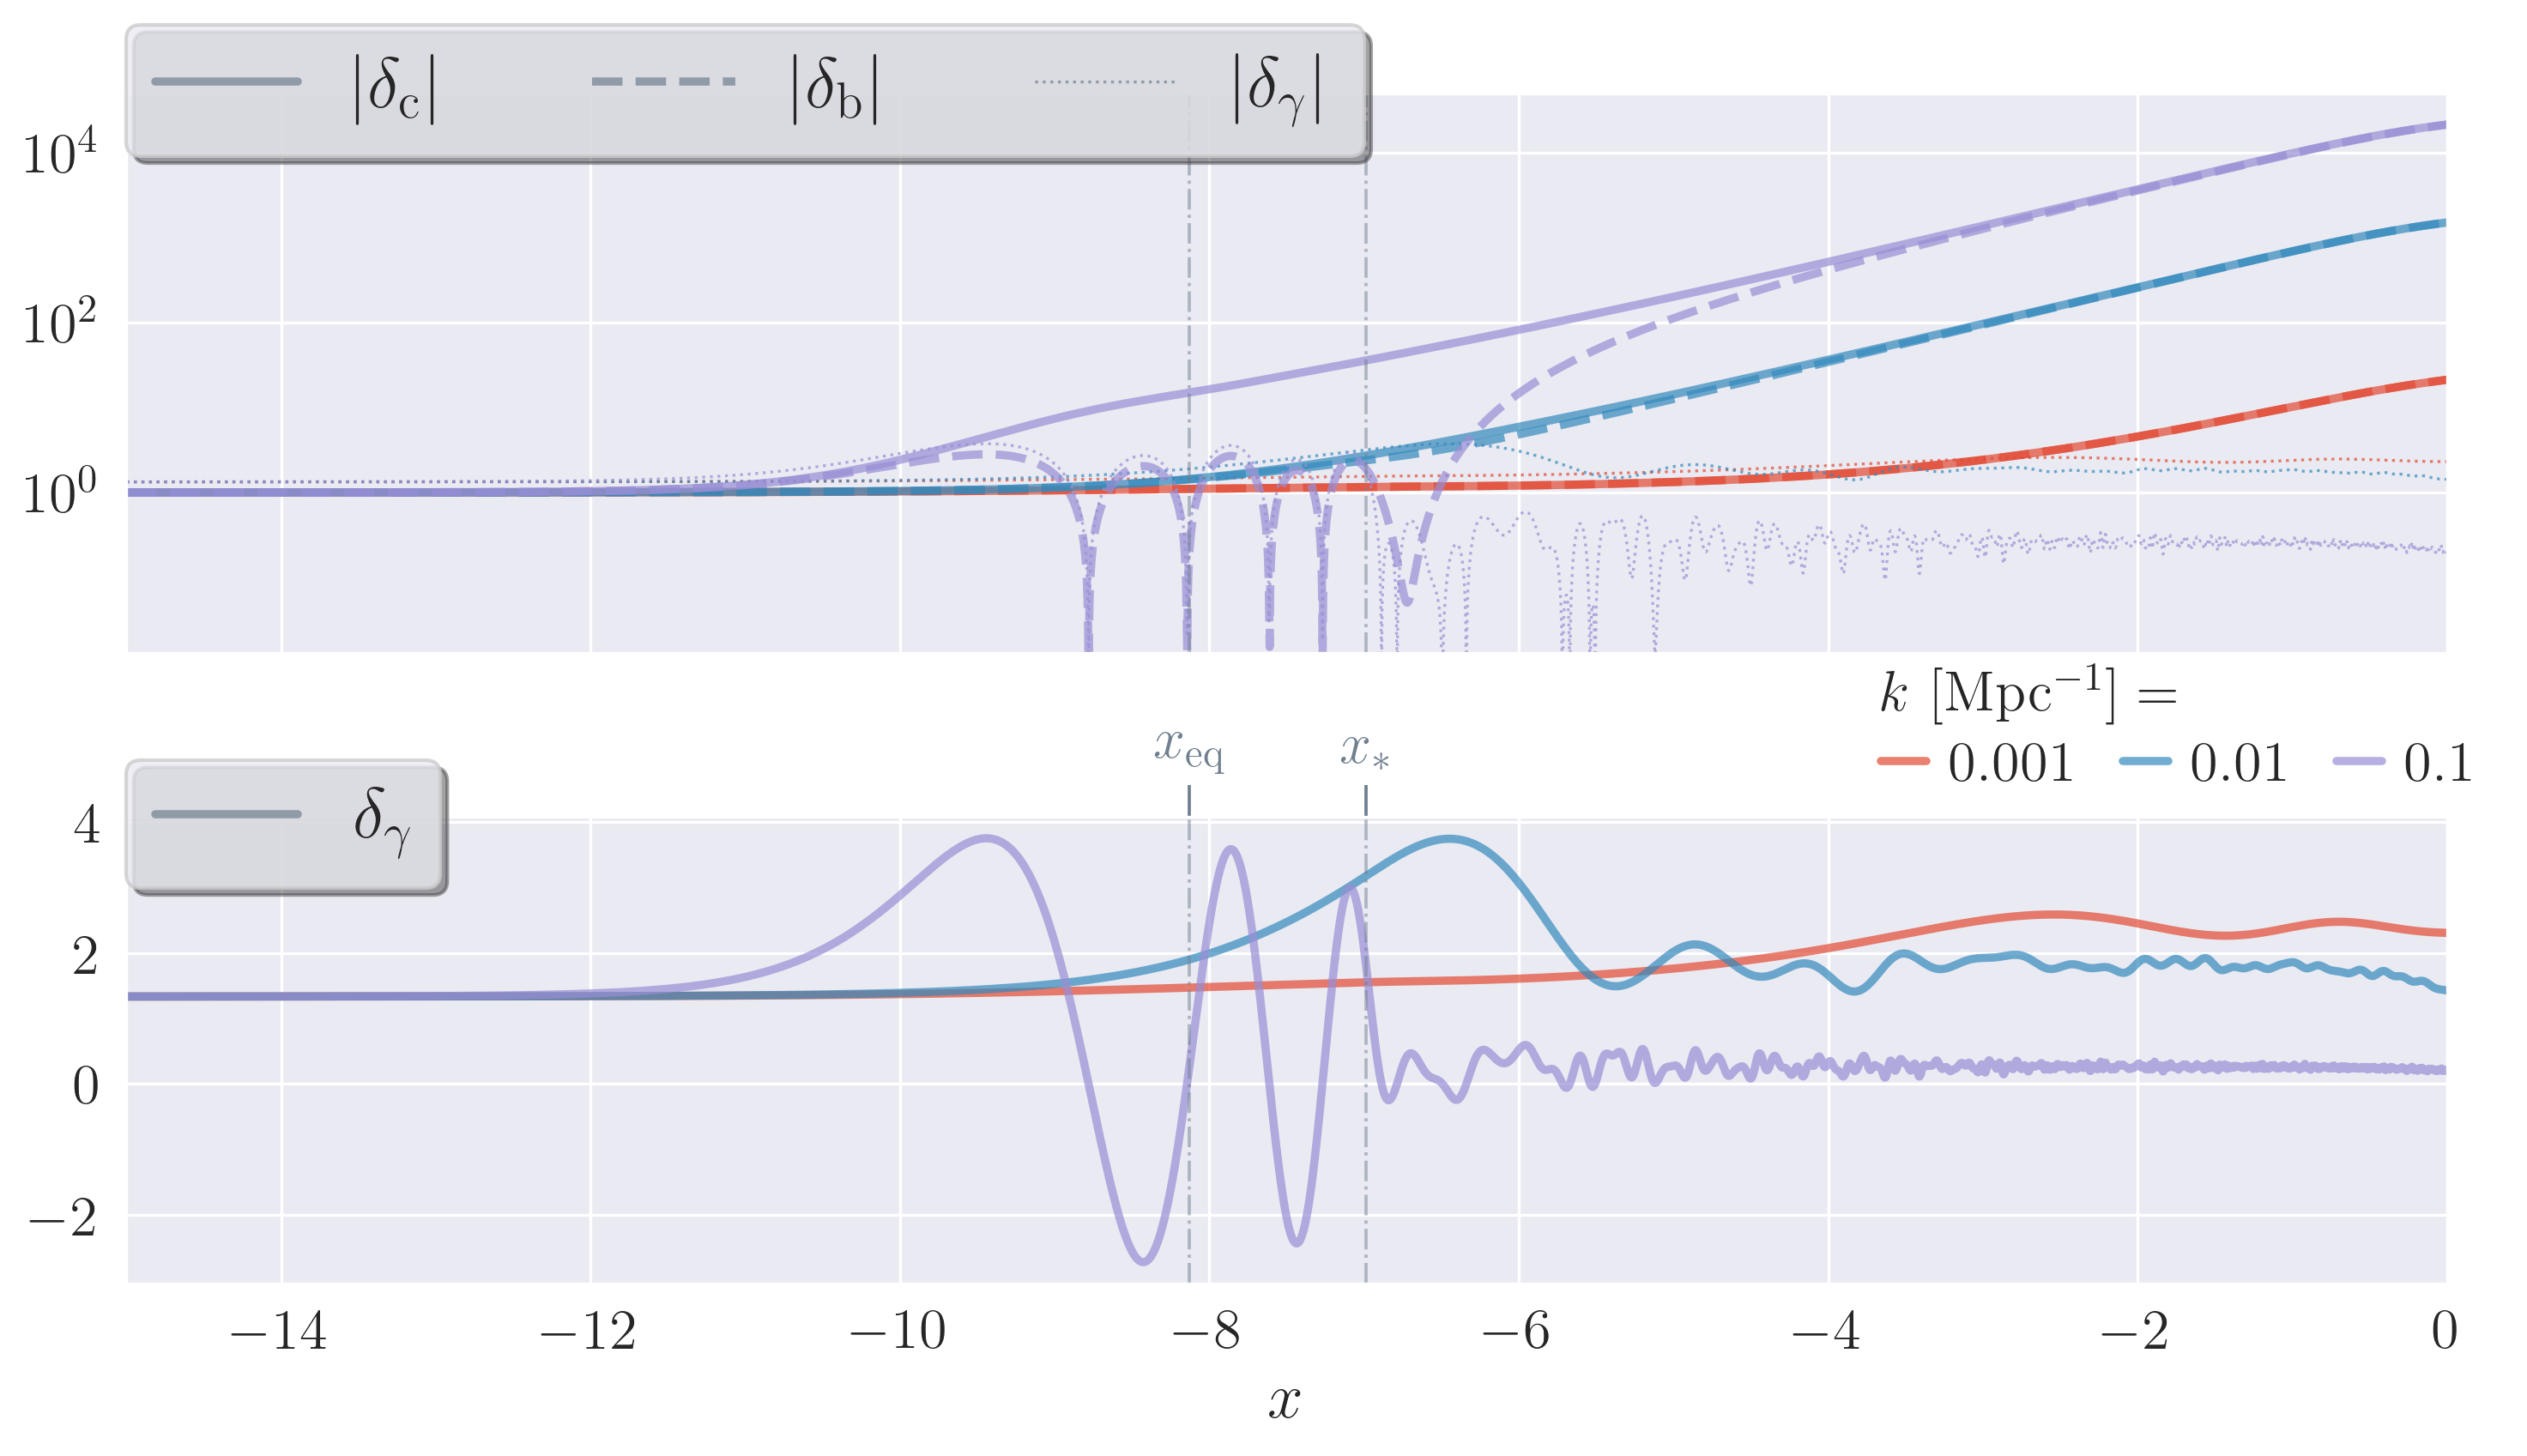
\includegraphics[width=\linewidth]{milestone3/density_perturbations.png} 
        \caption{Density perturbations $\delta_s(x, k)$ for $s=\mathrm{c,b}$ and $\gamma$ meaning cold dark matter, baryons and photons, respectively. Recall that $\delta_\gamma(x, k)=4\Theta_0(x, k)$.}
    \label[fig]{mil3:res:fig:density_perturbations}
    \end{subfigure} 
    \begin{subfigure}{0.49\linewidth}
        \centering
        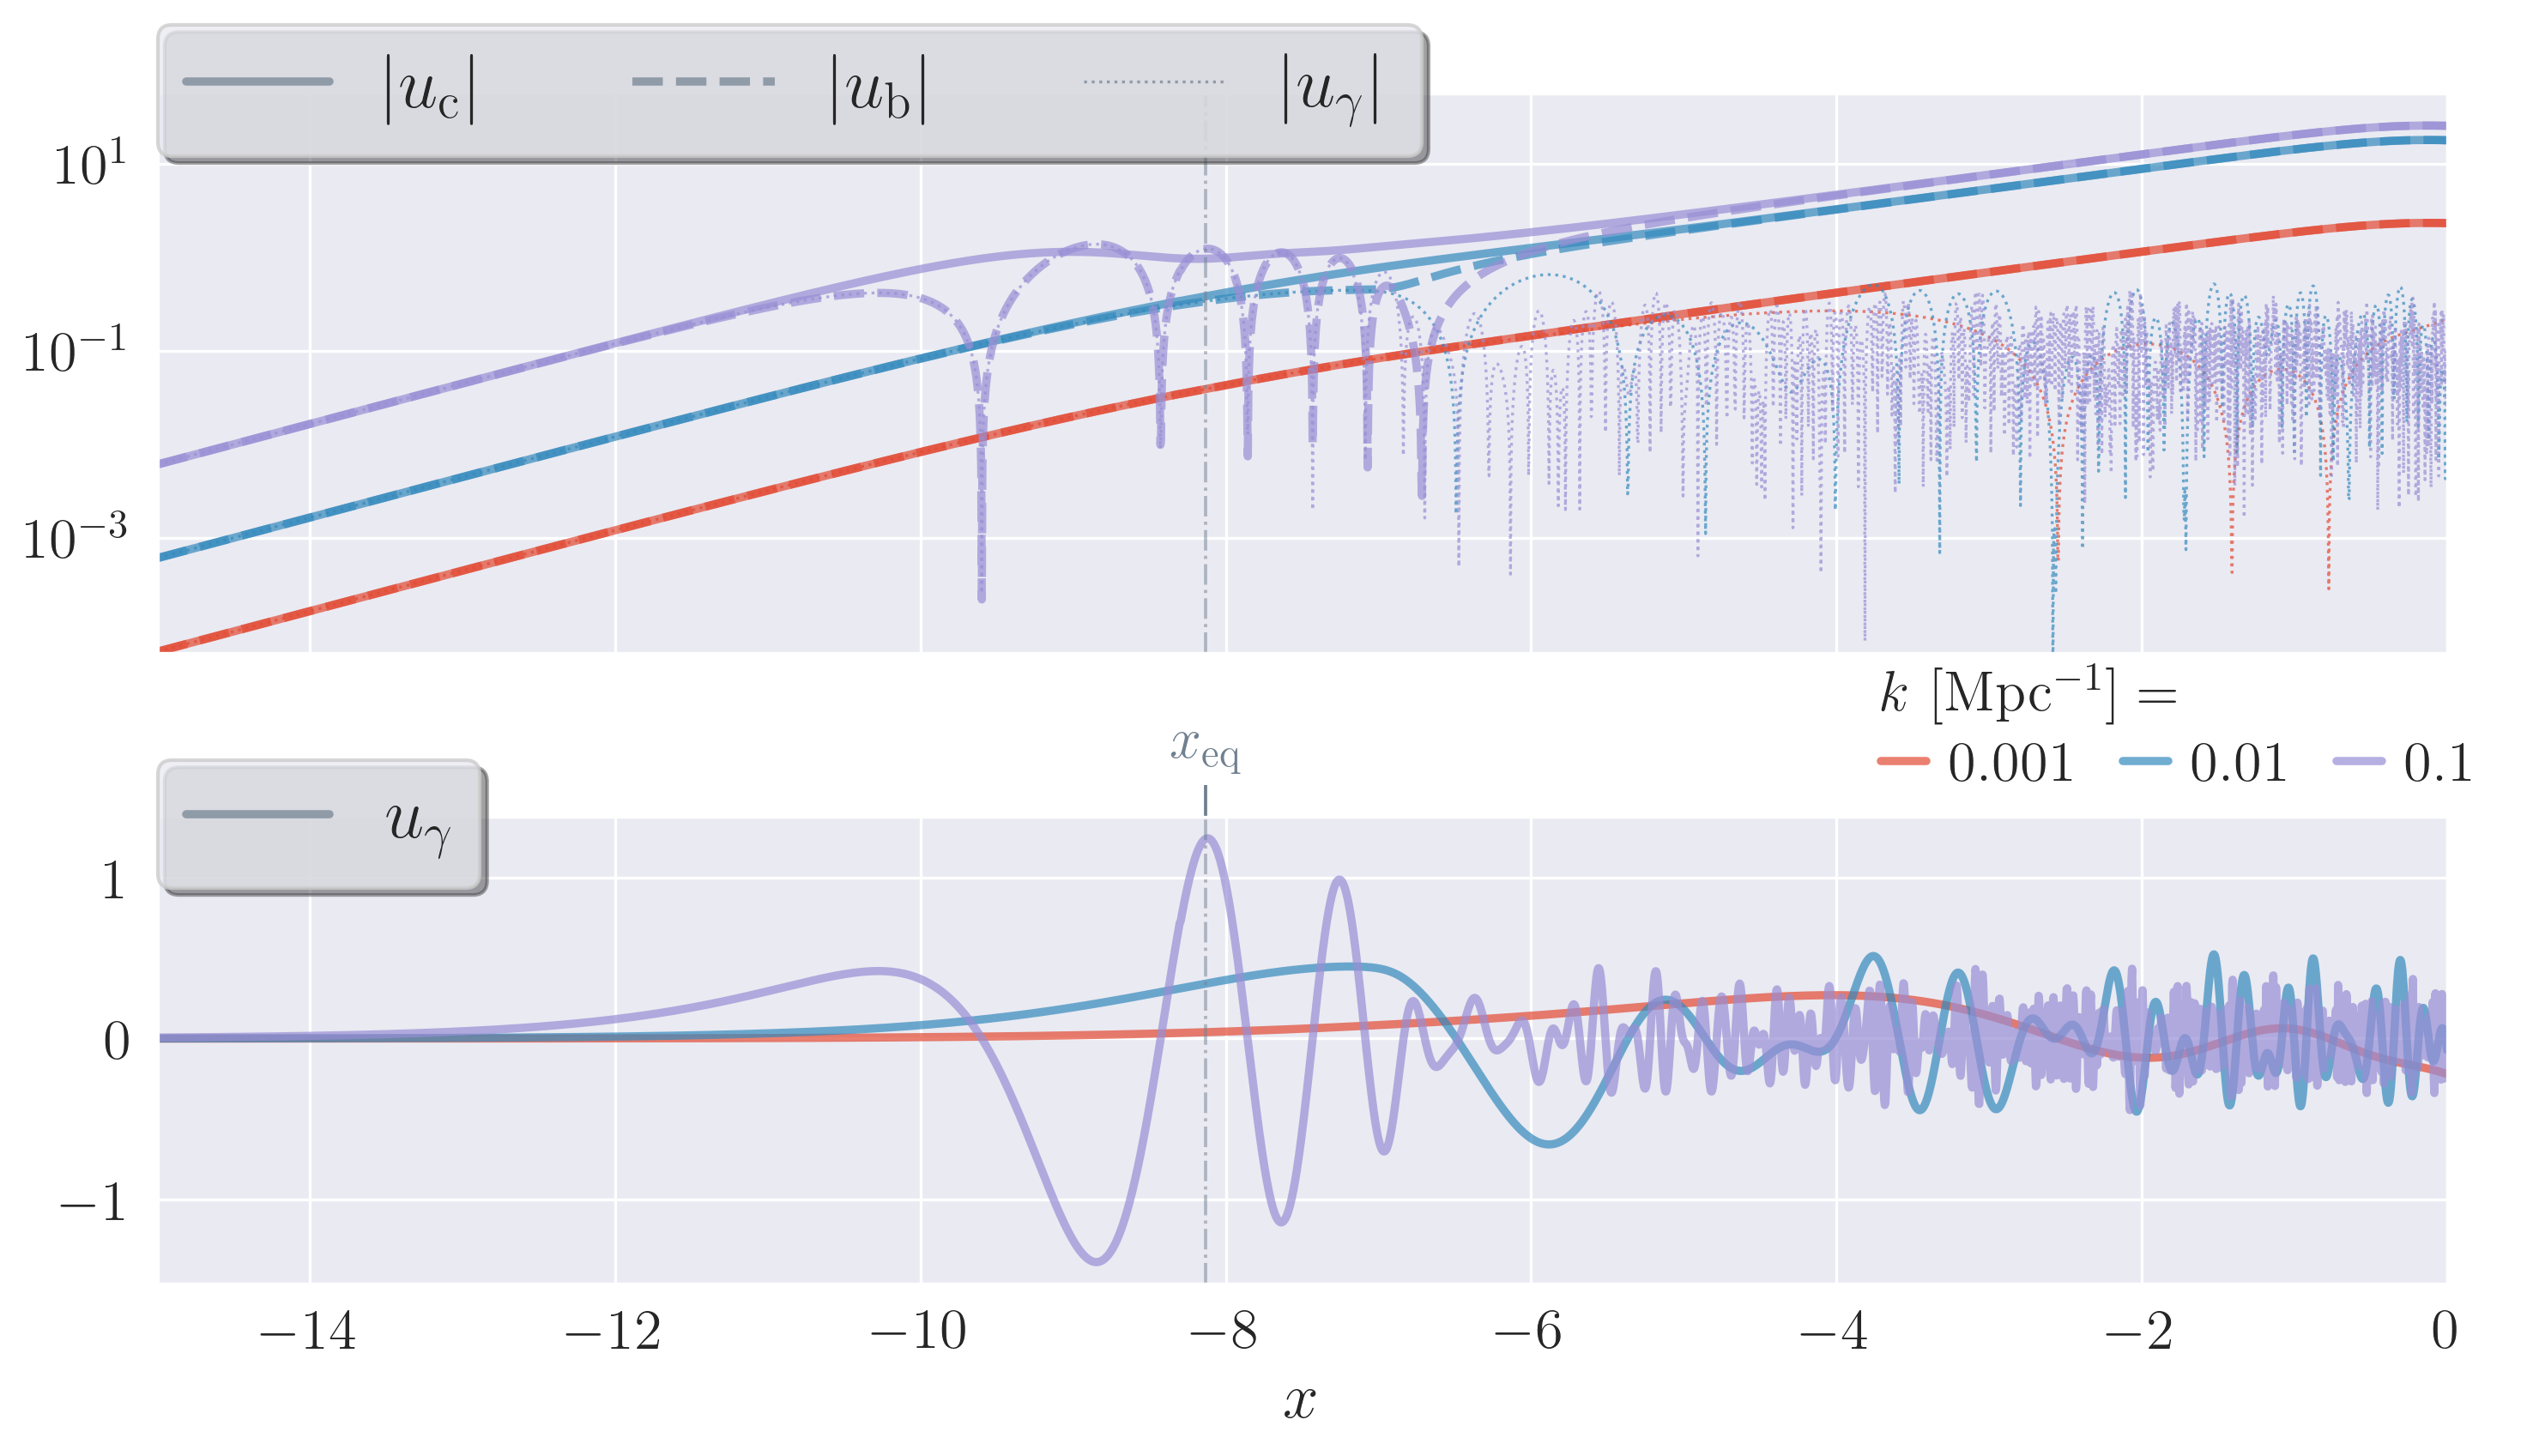
\includegraphics[width=\linewidth]{milestone3/velocity_perturbations.png} 
        \caption{Velocity perturbations $u_s(x, k)$ for $s=\mathrm{c,b}$ and $\gamma$ meaning cold dark matter, baryons and photons, respectively. Recall that $u_\gamma(x, k)=-3\Theta_1(x, k)$.} 
    \label[fig]{mil3:res:fig:velocity_perturbations}
    \end{subfigure}
    \caption{Matter perturbations to normal matter and photons as functions of logarithmic expansion $x$ for three wavenumbers $k$. The time of radiation-matter equality is emphasised by a shaded grey region, as is the recombination. Horizon entries are shown as thick, vertical coloured lines. The upper panels show the absolute value of the quantities in question with a logarithmic $y$-axes, whereas the lower panels show the actual quantity for the photons only.}
\label[fig]{mil3:res:fig:matter_perturbations}
\end{figure*}

The photon quadrupole is plotted in~\cref{mil3:res:fig:photon_quadrupole}. Note that the $x$-axis is relatively short in this plot, as the function is flat until $x\sim -9$.
\begin{figure}[!ht]
    \centering
    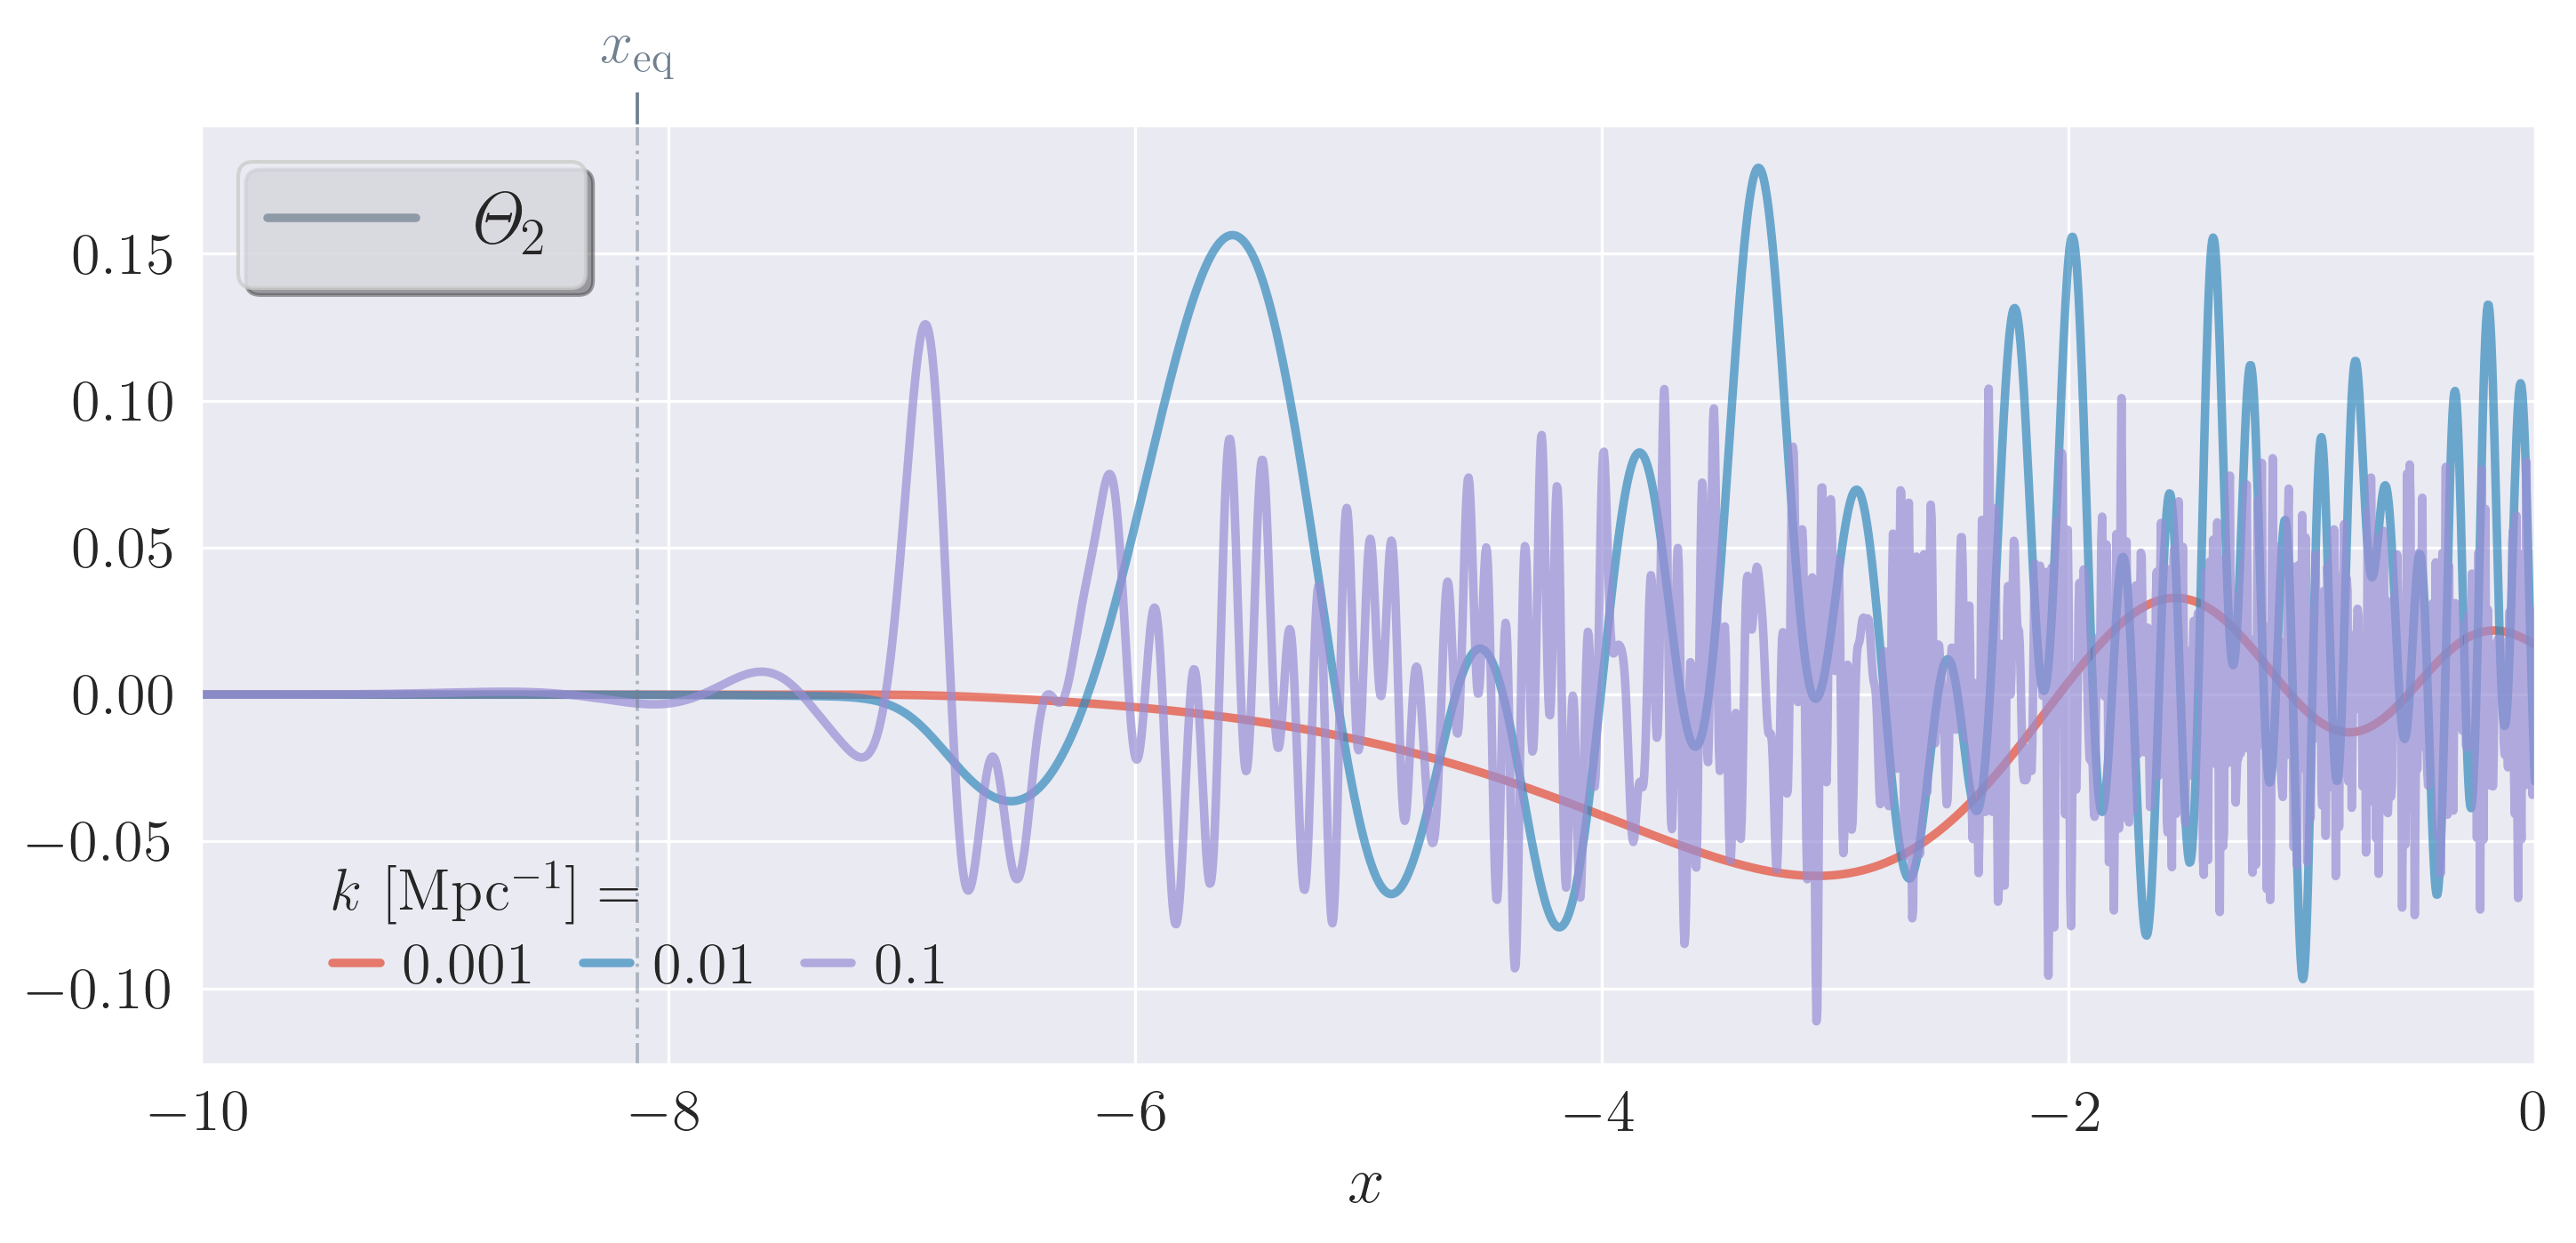
\includegraphics[width=\linewidth]{milestone3/photon_quadrupole.png} 
    \caption{The graphs show the photon quadrupole $\Theta_2(x, k)$ as function of logarithmic scale factor $x$ for three different wavenumbers $k$. The shaded grey regions represent the epochs of radiation-matter equality and recombination. Horizon entries are shown as thick, vertical coloured lines.} 
\label[fig]{mil3:res:fig:photon_quadrupole}
\end{figure}

\cref{mil3:res:fig:gravitational_potential} shows the scalar potentials as functions of time. The upper panel shows only the perturbation to the time-part of the metric, whereas the lower panel shows the sum of this and the spatial perturbation.
\begin{figure}[!ht]
    \centering
    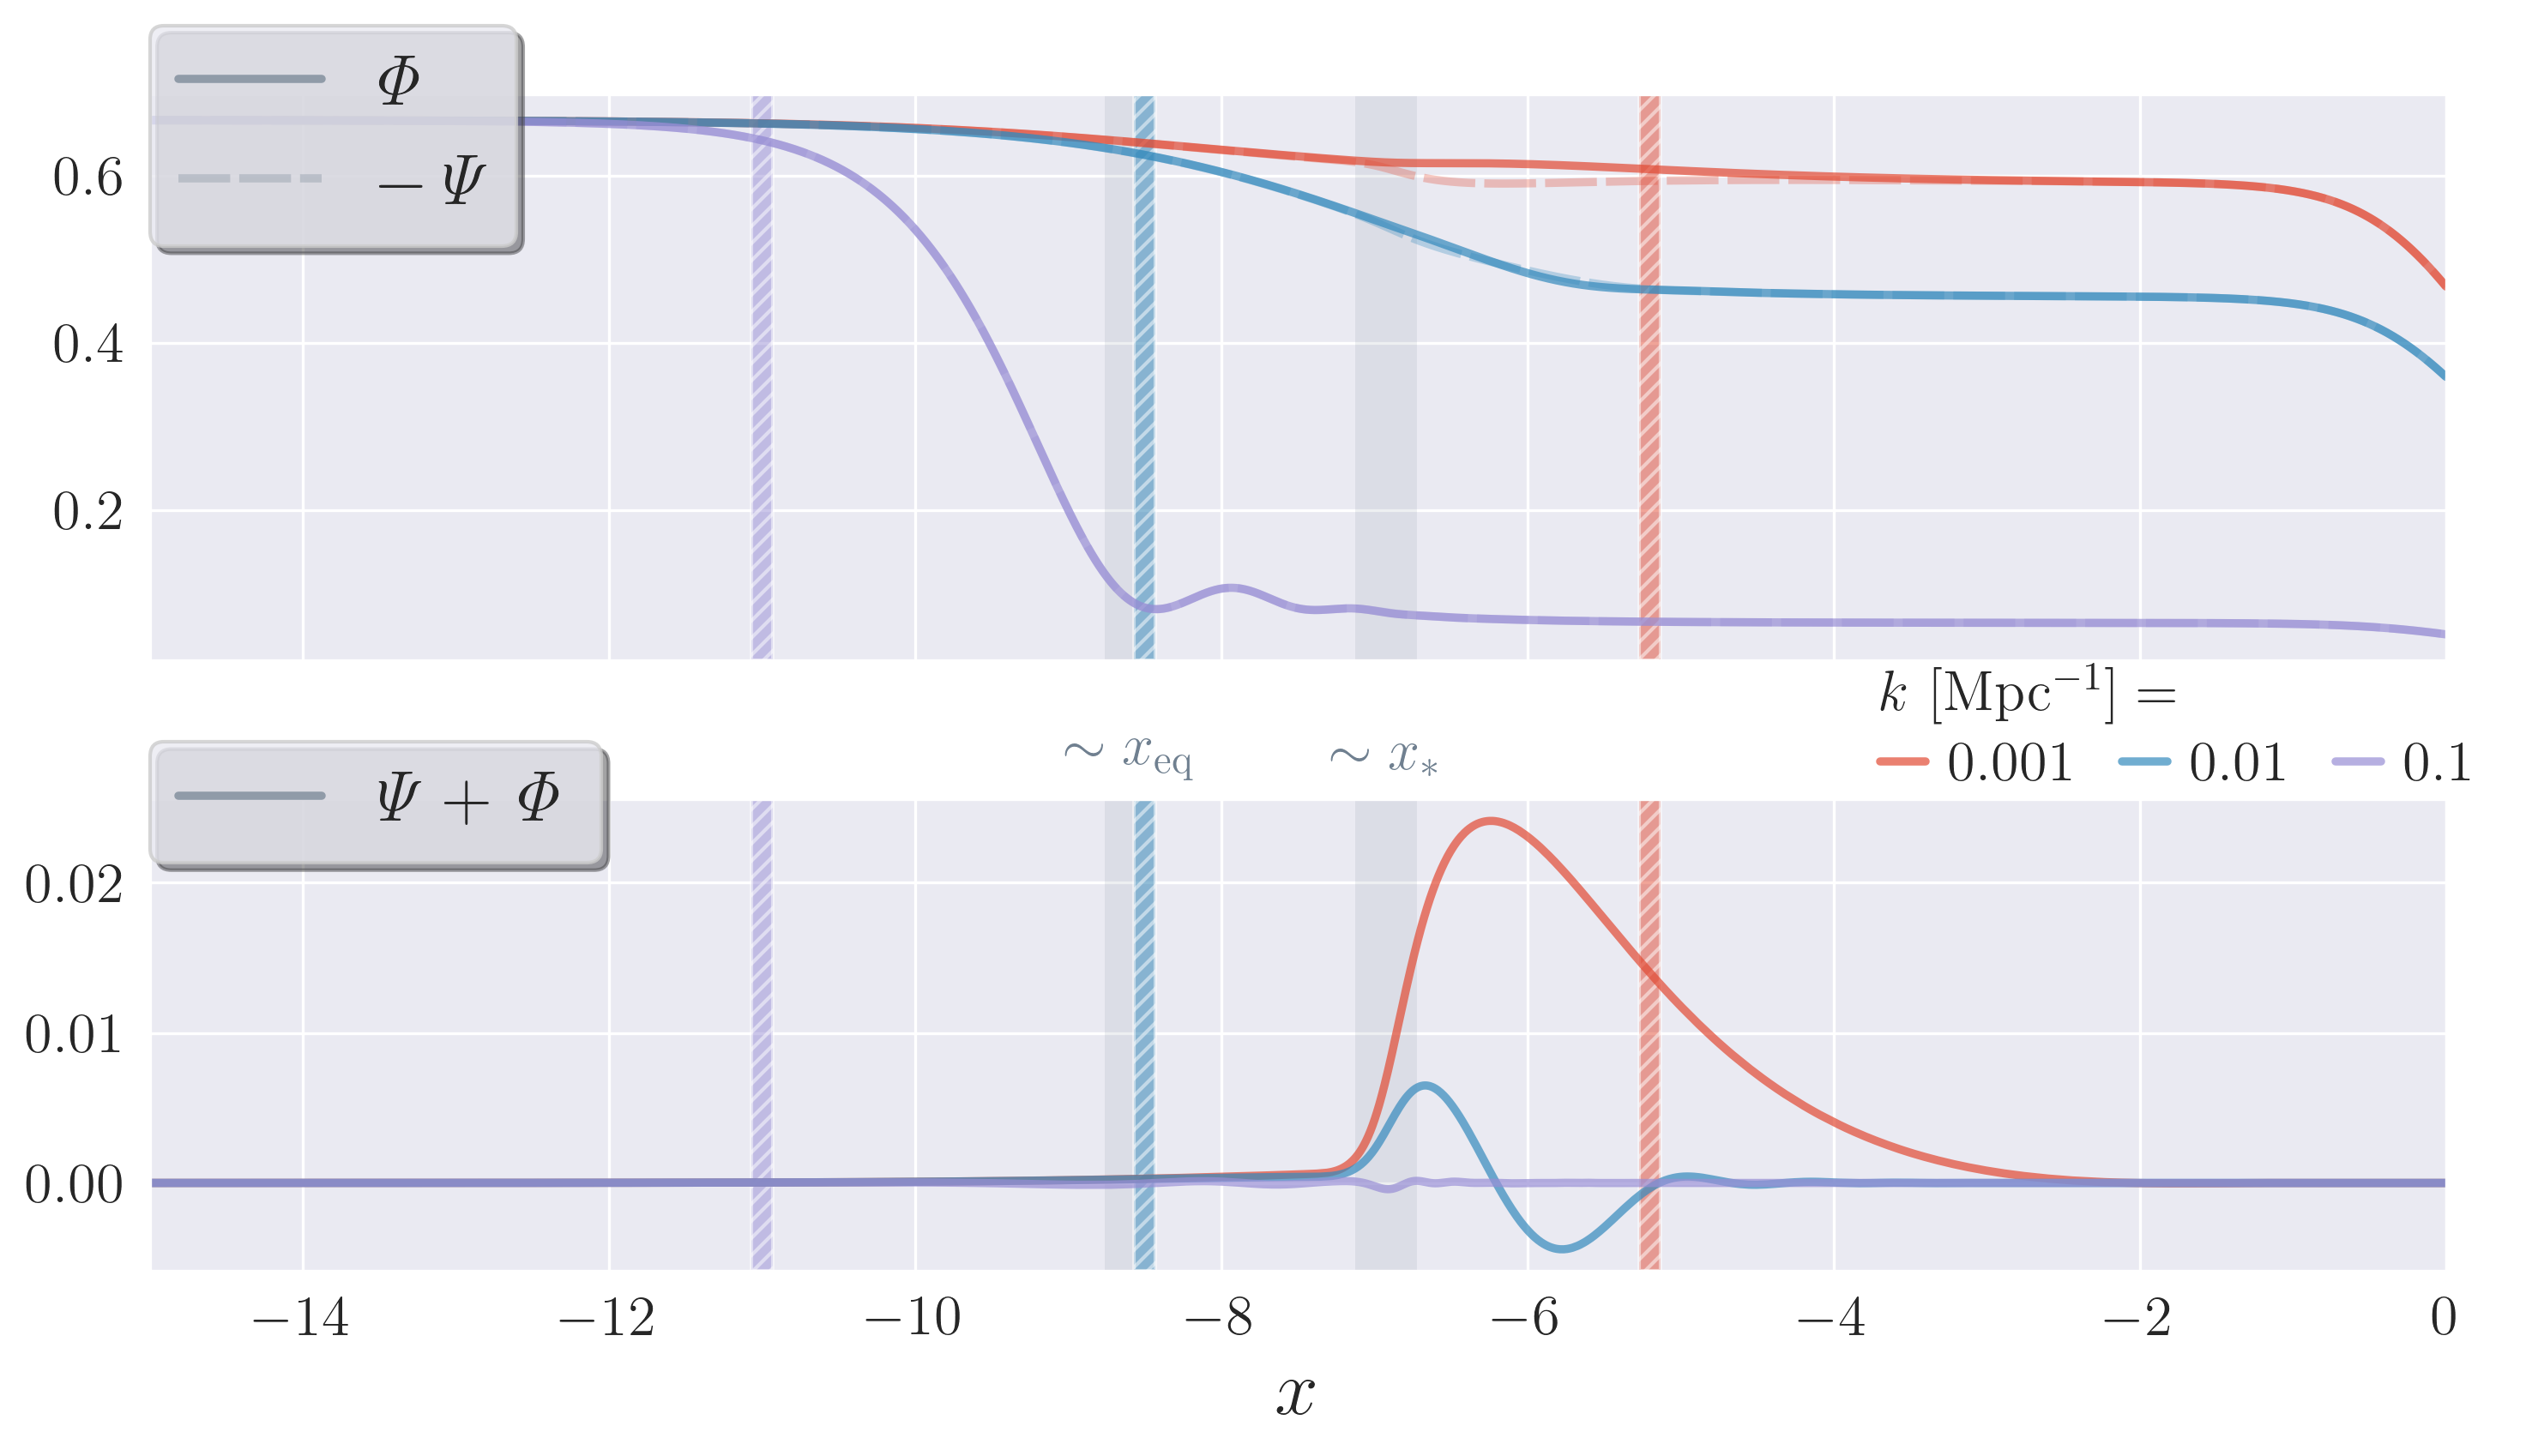
\includegraphics[width=\linewidth]{milestone3/gravitational_potential.png} 
    \caption{The graphs show the metric perturbations as functions of logarithmic scale factor $x$ for three different wavenumbers $k$. The shaded grey regions represent the epochs of radiation-matter equality and recombination. Horizon entries are shown as thick, vertical coloured lines. Upper panel: spatial curvature fluctuation $\Phi(x, k)$ and the negative gravitational potential $-\Psi(x, k)$. Lower panel: sum of the two potentials $\left(\Psi + \Phi\right)(x, k)$.} 
\label[fig]{mil3:res:fig:gravitational_potential}
\end{figure}

Note that we completely dismissed neutrinos and photon polarisation. That is, we sat the effective neutrino number to be zero, slightly changing the background from~\cref{sec:mil1}.

The end of tight coupling turned out to be $x\ped{tc,end}(k)=-8.3$ for all three wavenumbers. The three modes $k_s$, $k_i$ and $k_l$ entered the horizon at $x\sim -11$, $-8.5$ and $-5.2$, respectively. That is, $k_s$ enters the horizon in the radiation-dominated era, $k_i$ just around the radiation-matter equality and $k_l$ enters when the universe is dominated by matter (see~\cref{mil1:res:fig:density_params}; only now $x\ped{eq}=-8.66$). We decided to present updated details about the comoving wavenumbers we consider in a table;~\cref{mil3:res:tab:wavenumbers}. 
\begin{table}[h]
    \setlength\tabcolsep{0pt}
    \caption{The comoving wavenumbers we address, with their time of horizon entry (rightmost column).}
    \label[tab]{mil3:res:tab:wavenumbers}
    \begin{tabular*}{\linewidth}{@{\extracolsep{\fill}} l *{1}{d{1.4}} *{1}{d{3.3}} *{1}{d{3.3}} }
    \toprule
    % & \multicolumn{3}{c}{Time of event} \\
    & \multicolumn{1}{c}{$k\unit{[Mpc^{-1}]}$} & \multicolumn{1}{c}{$k/k_1$} & \multicolumn{1}{c}{$x\,| \,k\eta(x)\stackrel{!}{=}1$} \\
    \midrule
    $k_l$ ($\leadsto$ large scales)         & 0.001 & 0.052 & -10.98  \\
    $k_i$ ($\leadsto$ intermediate scales)  & 0.01  & 0.52 & -8.490  \\
    $k_s$ ($\leadsto$ small scales)         & 0.1   & 5.2 & -5.182  \\
    \midrule
    $k\ped{eq}$ ($\Rightarrow$ equality scale) & 0.0115 & 0.60 &  -8.658 \\
    \midrule
\end{tabular*}
\begin{tabular*}{\linewidth}{@{\extracolsep{\fill}} l r}
    Sound horizon at decoupling:     & $\sh = 164.0\unit{Mpc}$\\
    Fundamental mode:               & $k_1=\pi/\sh = 0.01916 \unit{Mpc^{-1}}$ \\
    \bottomrule
\end{tabular*}

% \begin{tabular*}{\linewidth}{@{\extracolsep{\fill}} l *{1}{d{1.4}} *{1}{d{3.3}} *{1}{d{3.3}} }
%     \toprule
%     % & \multicolumn{3}{c}{Time of event} \\
%     & \multicolumn{1}{c}{$k\unit{[Mpc^{-1}]}$} & \multicolumn{1}{c}{$k/k_1$} & \multicolumn{1}{c}{$x\,| \,k\eta(x)\stackrel{!}{=}1$} \\
%     \midrule
%     $k_l$ ($\leadsto$ large scales)         & 0.001 & 0.052 & -10.98  \\
%     $k_i$ ($\leadsto$ intermediate scales)  & 0.01  & 0.52 & -8.490  \\
%     $k_s$ ($\leadsto$ small scales)         & 0.1   & 5.2 & -5.182  \\
%     \midrule
%     $k\ped{eq}$ ($\Rightarrow$ equality scale) & 0.0115 & &  -8.658 \\
%     \midrule
% \end{tabular*}
% \begin{tabular*}{\linewidth}{@{\extracolsep{\fill}} l r}
%     Sound horizon at decoupling:     & $\sh = 164.0\unit{Mpc}$\\
%     Fundamental mode:               & $k_1=\pi/\sh = 0.01916 \unit{Mpc^{-1}}$ \\
%     \bottomrule
% \end{tabular*}
\end{table}

